\documentclass[12pt,letterpaper]{article}
\usepackage[utf8]{inputenc}
\usepackage[spanish,mexico]{babel}
\usepackage[top=2.5cm,bottom=2cm,left=1.8cm,right=2cm]{geometry}
\usepackage{graphicx}
\usepackage{caption}
\usepackage{amssymb}
\usepackage{floatrow}
\usepackage{fancyvrb}
\usepackage{xcolor}
\usepackage{xurl}
\usepackage{pgfgantt}

\PassOptionsToPackage{hyphens}{url}\usepackage{hyperref}
\hypersetup{
	colorlinks=true,
	urlcolor=blue,
	linkcolor=black
}

\pagestyle{headings}

\begin{document}
	\newgeometry{top=2cm,bottom=2.5cm,left=1cm,right=1cm}
	\begin{titlepage}
		\centering
		\begin{minipage}{0.14\linewidth}
			\includegraphics[width=\linewidth]{img/shieldUnam}
		\end{minipage}
		\begin{minipage}{0.7\linewidth}
			\centering
			{\bfseries\large UNIVERSIDAD NACIONAL AUTÓNOMA DE MÉXICO \par}
			%\vspace{1cm}
			\vfill
			{\scshape\Large Facultad de Ingeniería \par}
			\vfill
			%\vspace{0.7cm}
			{\scshape\Large Ingeniería en Computación \par}
		\end{minipage}
		\begin{minipage}{0.14\linewidth}
			\includegraphics[width=\linewidth]{img/shieldFi}
		\end{minipage}
		
		\centering
		\vspace{1.5cm}
		{\scshape\Large Bases de Datos \par}
		{\scshape\Large grupo: 01\par}
		\vspace{3cm}
		{\scshape\Huge Proyecto final \par}
		\vspace{0.8cm}
		%{\scshape\Huge fff \par}
		\vfill
		{\Large Alumnos: \par}
		\begin{center}
			\begin{tabular}{l}
				$\bullet$ {\Large Fonseca Huitrón Julise Aileen } \\
				\\
				$\bullet$ {\Large López Aniceto Saúl Isaac }\\
				\\
				$\bullet$ {\Large López González Kevin } \\
				\\
				$\bullet$ {\Large  Martínez Vázquez Diego}\\
				\\
				$\bullet$ {\Large Ponce Soriano Armando }\\
			\end{tabular}
		\end{center}
		\vfill
		{\Large Profesor: \par}
		{\Large ING. Fernando Arreola Franco \par}
		\vfill
		{\Large \today \par}
	\end{titlepage}
	
	\restoregeometry
	\tableofcontents
	
	\newpage
	\section{Introducción}
	Este proyecto consiste en elaborar el diseño y la creación de una base de datos que utilizará una cadena de papelerías en la que se puede manipular y almacenar la información de todos los productos que esta cadena ofrece. Esta base de datos tendrá como finalidad llevar de manera ordenada y controlada la logística que la papelería sigue para tener control de todos los servicios que ofrece, así como llevar un control de las transacciones y accesos. 
	\\
	\\ Para su correcta manipulación se contempla la creación de una página web, que le permita a los usuarios  acceder de manera fácil y rápida a las funciones que se desarrollaron en la base de datos y se pueda ver de una forma gráfica. . 
	\\
	\\El desarrollo de esta base de datos será detallado en el presente documento con la finalidad de explicar los procedimientos, planes y metodologías que se fueron utilizadas para llevar a cabo este proyecto. 
	\\
	\\Este proyecto fue elaborado en POSTGRESQL, utilizando los recursos de PHP y AmazonWebServices
	
	
	\section{Plan de trabajo}\\
	A continuación, se describe el plan de trabajo utilizado para el desarrollo de este proyecto, principalmente consiste en asignar tareas específicas a todos los participantes, con base en el establecimiento de metas y fechas.
	
	\subsection{Descripción}
	Debido a la magnitud y características del proyecto se decidió utilizar una metodología ágil, que permitiera cumplir con todos los requerimientos del cliente.
	Por sus cualidades, Scrum fue la mejor alternativa, ya que, nos permitió:
	
	\begin{itemize}
		\item Definir el Product Backlog:  ordenar de mayor a menor importancia las funcionalidades pedidas por el cliente. 
		
		\item Desarrollar la lista de tareas de la iteración o Sprint Backlog.
		
		\item Realizar Sprint Planning Meeting a lo largo del Sprint Backlog con el equipo de trabajo para determinar el enfoque del proyecto, las etapas y los plazos.
		
		\item Durante todo el periodo de Sprint, realizar reuniones con el equipo encargado para conocer los avances, las tareas por terminar y las necesidades para terminar dichas tareas.
		
		\item Al concluir con los Sprint, realizar el Sprint Review, para revisar todos los avances del proyecto
		
	\end{itemize}
	
	
	\subsection{Plan de actividades}
	
	\\En el siguiente cronograma se podrá consultar los Sprint estableciendo para la creación y desarrollo del sistema, estableciendo fechas y un límite de tiempo para cada tarea.\\ 
	\\En la parte de asignaciones, se destina cada uno de los integrantes una tarea referida en el cronograma y que forma parte de la elaboración de este proyecto. \\
	
	\subsection{Cronograma}
	\begin{figure}[H]
		\centering
		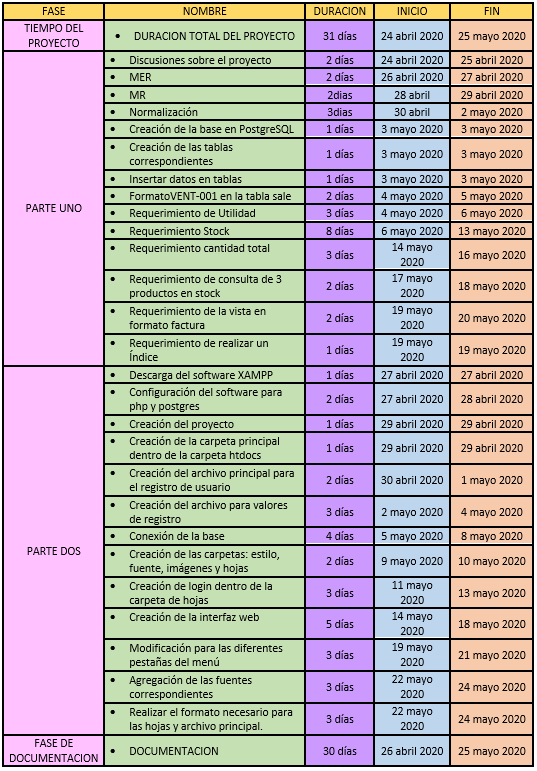
\includegraphics[scale=1.00]{Documentacion/img/cronograma.PNG}
		\caption{Cronograma}
	\end{figure}
	
	
	\subsection{Aportaciones}
	\begin{center}
		\begin{tabular}{c|c|c|c|c|c}
			& Diseño & Implementación & Presentación & Acoplamiento & Documentación\\ \hline
			Fonseca Huitrón Julise & $\checkmark$ &$\checkmark$ & & & $\checkmark$ \\
			López Aniceto Isaac & $\checkmark$ & $\checkmark$ & & \\
			López González Kevin & $\checkmark$ & & $\checkmark$ & $\checkmark$ & $\checkmark$\\
			Martínez Vázquez Diego& $\checkmark$ & $\checkmark$ &  &  & $\checkmark$\\
			Ponce Soriano Armando & $\checkmark$ & & $\checkmark$ & $\checkmark$ 
		\end{tabular}
	\end{center}
	
	\section{Diseño}
	\subsection{Análisis de requerimientos}
	\\Para la elaboración de la base de datos se contempla que una papelería tendrá una serie de registros que a su vez contendrán información, se requiere almacenar información de los proveedores, se requiere almacenar información sobre un Inventario que almacena también información. Se deberá guardar información detallada de cada venta realizada.\\
	\\Requerimos también toda la información relacionada con el cliente y también información específica del o los tipos de producto que tenemos a la venta.\\
	\\Los requerimientos antes mencionados nos llevan a conceptualizar más las ideas, encontrando que hay dependencias en algunos de ellos, nos lleva a analizar la cardinalidad que hay entre las tablas.\\
	\\El análisis de estos requerimientos es la base para la construcción de nuestros modelo Entidad-Relación y en general de todo el modelo Conceptual. 
	
	
	\subsection{Modelo conceptual}
	\textbf{Entidades}\par 
	\begin{itemize}
		\item PROVEEDOR: \{ \underline{id\_Proveedor}, razón social, domicilio (estado, código postal, colonia, calle y número), nombre, teléfonos \}
		\item CLIENTE: \{\underline{RFC}, nomre (nombre, ap\_Paterno, ap\_Materno), domicilio (estado, código postal, colonia, calle y número), emails \}
		\item INVENTARIO: \{\underline{id\_Inventario}, precio\_compra, fecha\_compra, cantidad\_ejemplares \}
		\item PRODUCTO: \{\underline{código\_Barras}, marca, descripción, precio, categoria\}
		\item VENTA : \{\underline{num\_venta}, fecha\_venta, pago\_Total, cantidad\_articulo, pago\_total\_Articulo \}
	\end{itemize}
	
	\textbf{Relaciones}\par
	\begin{itemize}
		\item Un proveedor surte a muchos inventarios.
		\item Un inventario es surtido por muchos proveedores.\\
		\item Un inventario almacena muchos productos.
		\item Un producto es almacenado por un inventario.\\
		\item Una venta contiene muchos productos.
		\item Un producto es contenido es muchas ventas.\\
		\item Un cliente concreta muchas ventas.
		\item Una venta es concretada por un cliente.
		
	\end{itemize}
	\subsubsection{Modelo Entidad-Relación}
	\begin{figure}[H]
		\centering
		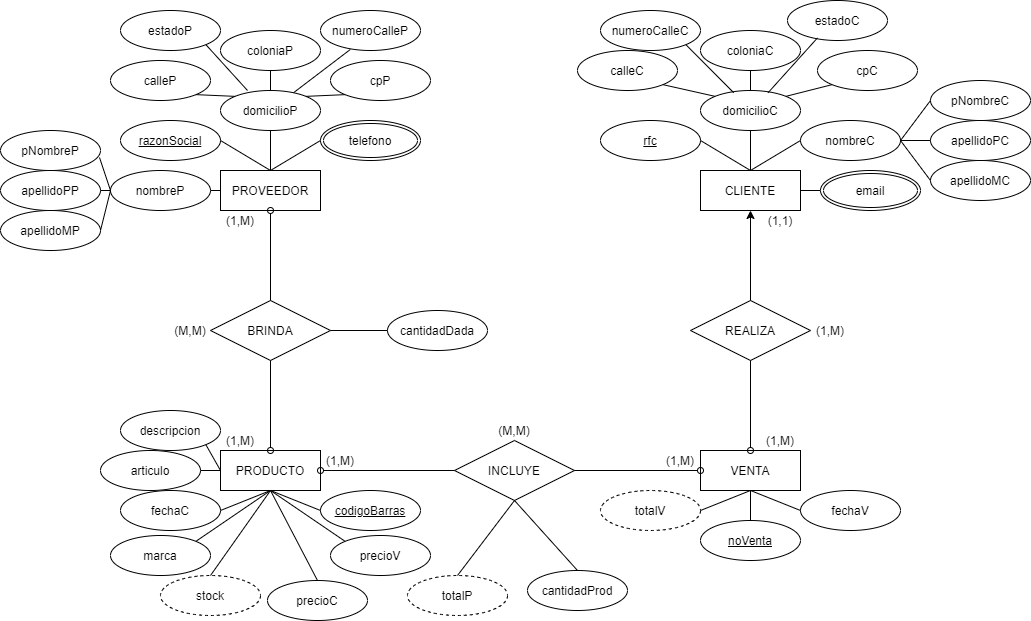
\includegraphics[width=\linewidth]{img/MER.png}
		\caption{Modelo Entidad-Relación.}
	\end{figure}
	
	
	\subsection{Modelo lógico}
	\subsubsection{Representación Intermedia}
	Realizando el Modelo Entidad-Relación, pudimos seguir las reglas para de la transformación de MER a MR, nos derivó en las siguientes tablas:
	\begin{itemize}
		\item PROVEEDOR: \{ id\_proveedor smallint (PK), nombre varchar 50, razón social varchar 50, estado varchar 50, colonia varchar 50, numero smallint, cp smallint, calle varchar 50\}
		
		\item TELEFONO: \{teléfono bigint(PK), id\_proveedor smallint (FK)\}
		
		\item INVENTARIO: \{id\_Inventario smallint (PK), nombre varchar(50)\}
		
		
		\item SURTE: \{[id\_Provedor smaillint (FK), id\_Inventario smallint (FK)] (PK)\}
		
		\item PRODUCTO: \{cod\_barras integer PK, id\_categoria smallint FK, precio smallint NOT NULL, marca varchar(20) NOT NULL, descripcion varchar(50)\}
		
		\item CATEGORÍA: \{ id\_categoria smallint PK, tipo varchar(20) NOT NULL\}
		
		\item GUARDA: \{[id\_Inventario smallint (FK), cod\_Barras int(FK)] (PK), dateprecio\_compra decimal (10,2), stock smallint, fecha\_compra date\}
		
		\item CLIENTE: \{RFC varchar(13) (PK), nombre varchar(20), ap\_paterno varchar (20), ap\_materno varchar (20) (N), cp smallint, numero smallint, estado varchar (32), calle varchar (32), colonia varchar (32)\}
		
		\item EMAIL: \{RFC varchar(13) (FK), email varchar (64) (PK)\}
		
		\item VENTA: \{id\_venta int(PK), fecha\_venta date, pago\_final decimal(7,2), RFC varchar(13)(FK)\}
		
		\item CONTIENE: \{ [cod\_barras int , id\_venta int](PK)(FK), precioTotalArt decimal(7,2), cantidad articulo int\} 
	\end{itemize}
	
	\subsubsection{Transformación de MER a MR}
	Para la transformación de Modelo Entidad Relación a Modelo Relacional, primero debemos utilizar la transformación intermedia que obtuvimos y desarrollamos. Una vez finalizado ese procedimiento utilizamos las reglas para la trasformación de MER a MR y obtendremos nuestro modelo relacional.  
	
	\subsubsection{Modelo Relacional}
	\begin{figure}[H]
		\centering
		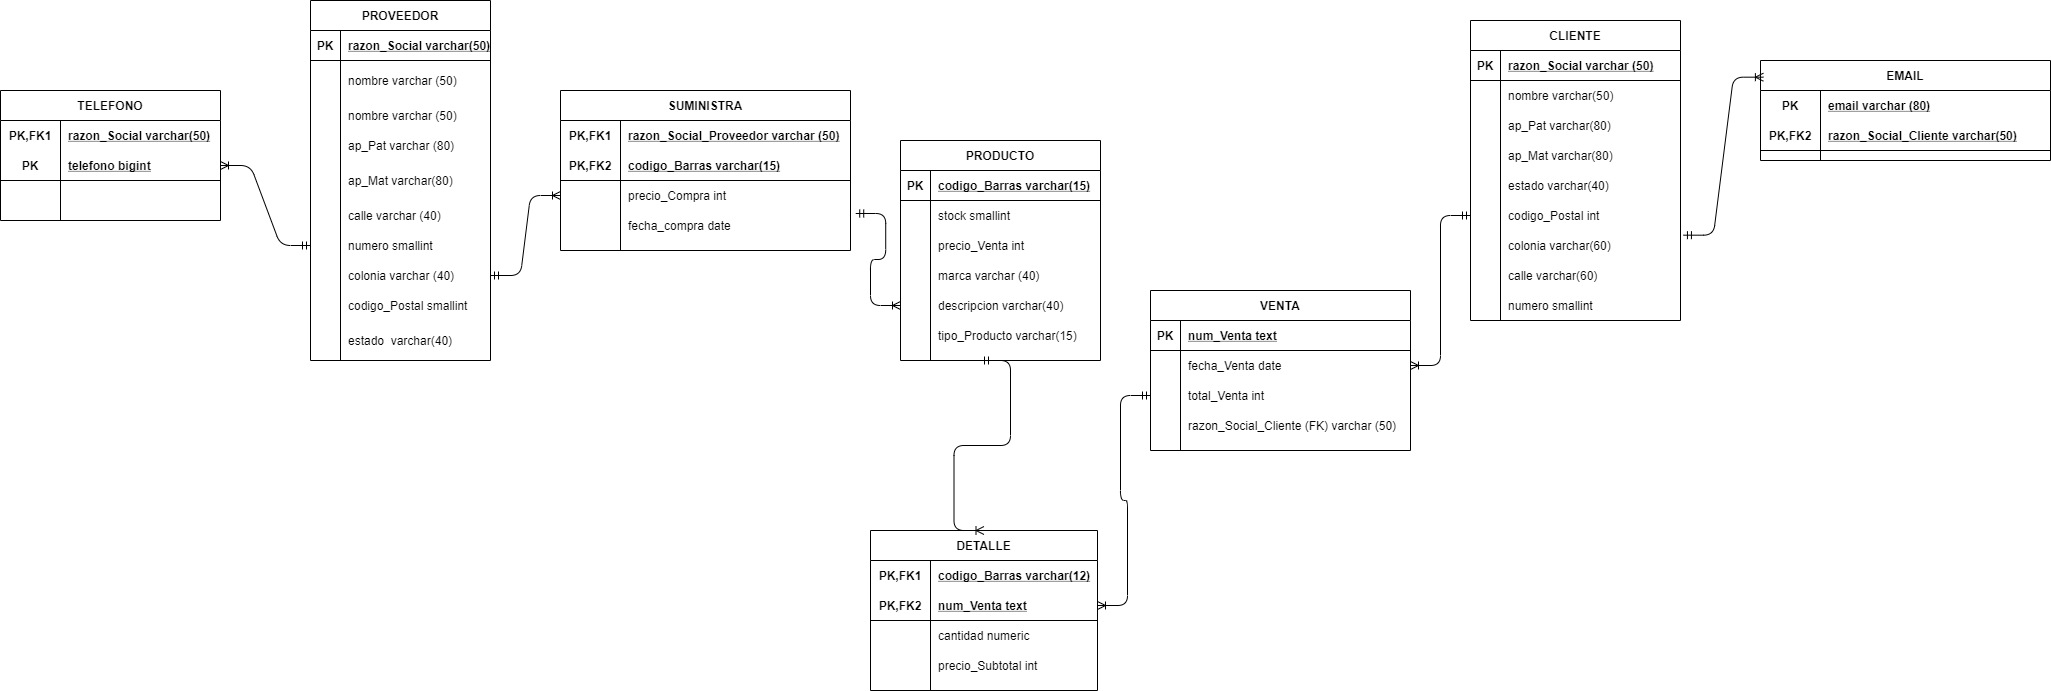
\includegraphics[width=\linewidth]{img/MR.png}
		\caption{Modelo Relacional.}
	\end{figure}
	
	\subsubsection{Normalización}
	
	Se cumple con la 1FN, ya que las tablas no presentan grupos de repetición y cada columna contiene valores atómicos.\\
	\\
	Correo:cumple la 2FN debido a que PK es simple.
	\\ email $\rightarrow$ RFC \\
	\\ Cliente: cumple la 2FN debido a que PK es simple.
	\\ RFC $\rightarrow$ {nombre, ap\_Paterno, ap\_Materno, cp, estado, calle, colonia}\\
	\\ Venta: cumple la 2FN debido a que PK es simple
	\\ id\_Venta $\rightarrow${fecha\_Venta, pago\_Final, RFC}\\
	\\ Contiene: No existen dependencias funcionales parciales
	\\ {cod\_Barras, id\_Venta} $\rightarrow$ {precio\_Total,cantidad\_Articulo}\\
	\\Producto: cumple la 2FN debido a que PK es simple.
	\\Cod\_Barras $\rightarrow$ {precio, marca, descripción, id\_Categoia}\\
	\\Categoría: cumple la 2FN debido a que PK es simple.
	\\id\_Categoria $\rightarrow$ tipo\\
	\\Inventario: cumple la 2FN debido a que PK es simple.
	\\id\_Inventario $\rightarrow$ nombre\\
	\\Guarda: No existen dependencias funcionales parciales
	\\{id\_Venta, cod\_Barras} $\rightarrow$ {precio\_Compra, stock, fecha\_Compra}\\
	\\Proveedor: cumple la 2FN debido a que PK es simple.
	\\Id\_Proveedor: nombre, razón\_Social, estado, colonia, numero, cp, cale \\
	\\Teléfono:
	\\num\_Telefono $\rightarrow$id\_Proovedor\\
	
	\\Se cumple con la 3FN, ya que se cumple con la 2FN y no hay transitividad en las tablas\\
	
	\section{Implementación}
	Para llevar a cabo la implementación de esta base de datos, primero tendremos que crear la base de datos en el manejador POSTGRESQL.\\
	\\Una vez finalizada la creación de la base de datos, tendremos que crear las tablas que obtuvimos en nuestro modelo relacional. Estas tablas tendrán que tener sus respectivos constraints para las llevas primarias y foráneas que se utilizan en toda la base de datos.\\
	\\Cuando las tablas estén creadas en las base de datos, podremos verificar su utilidad haciendo inserciones de prueba. \\
	\\Para que el sistema resuelva cuando se reciba un código de barras regrese la utilidad, para que cuando haya la venta de un artículo y se decremente el stock por la cantidad vendida, dada una fecha o una fecha de inicio y de fin, regrese la cantidad total que se vendió y su ganancia correspondiente.  Para obtener el nombre de aquellos productos que están es stock, que de forma automática genere vista que contenga información para desplegar una factura de compra y la creación del índice. Para todas esas funciones mencionadas, tendremos que hacer uso de la creación de Functions, Procedures y Triggers. 
	
	\subsection{Modelo físico}
	
	\subsubsection{IaaS}
	La infraestructura como servicio (IaaS) es un método que ofrece la funcionalidad de almacenar información a través de Internet.\\
	\\Amazon Web Services (AWS) es la plataforma en la nube más adoptada y completa, permitiendo reducir costos, aumentar su agilidad e innovar de forma más rápida, además de su disponibilidad las 24 horas del día.\\
	
	\begin{figure}[H]
		\centering
		\includegraphics[width=\linewidth]{Documentacion/img/iaas.PNG}
		\caption{IaaS.}
	\end{figure}
	\\Debido a diferentes circunstancias sucitadas durante el desarrrollo del proyecto, se tuvo que optar por el uso de una base de datos de forma local, aunque es importante aclararar que se lograron conexiones exitosas con una base de datos en la nube mediante estos servicios.\\
	
	\subsection{DDL}
	\\El lenguaje de definición de datos (Data Definition Language), permite definir las estructuras que almacenarán los datos, así como los procedimientos o funciones que permitan consultarlos.
	
	
	La tabla cliente, permite guardar todos sus datos;  debido a que un RFC nunca se repite se  usara para comunicarse con las tablas Correo y Venta. 
	En la siguiente tabla 
	\begin{figure}[H]
		\centering
		\includegraphics[scale=0.90]{Documentacion/img/tablaCliente.PNG}
		\caption{Tabla Cliente.}
	\end{figure}
	Con la implementación de la tabla Correo el cliente podrá proporcionar al menos un correo. 
	\begin{figure}[H]
		\centering
		\includegraphics[scale=0.90]{Documentacion/img/tablaCorreo.PNG}
		\caption{Tabla Correo.}
	\end{figure}
	La tabla Venta contiene los datos más generales de dicha acción. 	
	\begin{figure}[H]
		\centering
		\includegraphics[scale=0.90]{Documentacion/img/tablaVenta.PNG}
		\caption{Tabla Venta.}
	\end{figure}
	La siguiente tabla tiene los datos generales del producto vendido, es por eso que se relaciona con la tabla anterior y posterior. 
	\begin{figure}[H]
		\centering
		\includegraphics[scale=0.90]{Documentacion/img/tablaVenta.PNG}
		\caption{Tabla Venta.}
	\end{figure}
	En la tabla Producto se guardan los datos particulares de cada uno de estos.	
	\begin{figure}[H]
		\centering
		\includegraphics[scale=0.90]{Documentacion/img/tablaProducto.PNG}
		\caption{Tabla Venta.}
	\end{figure}
	Debido a que los productos son diversos, los seccionamos en cuatro categorías (regalos, papelería, impresiones y recargas), es por ello que establecemos un id para identificar a cada una. 	
	\begin{figure}[H]
		\centering
		\includegraphics[scale=0.90]{Documentacion/img/tablaCategoria.PNG}
		\caption{Tabla Categoría.}
	\end{figure}
	La tabla que se muestra a continuación permitirá tener los detalles particulares de la venta. 	
	\begin{figure}[H]
		\centering
		\includegraphics[scale=0.90]{Documentacion/img/tablaGuarda.PNG}
		\caption{Tabla Guarda.}
	\end{figure}
	Con el inventario se podrá tener acceso y control dela información referente a la venta. 	
	\begin{figure}[H]
		\centering
		\includegraphics[scale=0.90]{Documentacion/img/tablaInventario.PNG}
		\caption{Tabla Inventario.}
	\end{figure}
	La tabla Surte permitirá comunicar al inventario con el proveedor. 	
	\begin{figure}[H]
		\centering
		\includegraphics[scale=0.90]{Documentacion/img/tablaSurte.PNG}
		\caption{Tabla Surte.}
	\end{figure}
	Finalmente, esta tabla podrá tener el número telefónico de varios proveedores 	
	\begin{figure}[H]
		\centering
		\includegraphics[scale=0.90]{Documentacion/img/tablaTelefono.PNG}
		\caption{Tabla Telefono.}
	\end{figure}
	En el siguiente apartado, se podrán consultar las modificaciones realizadas a las tablas para su correcta conexión, usando las llaves primarias y foráneas, de acuerdo a lo establecido en el MR. 
	
	\begin{figure}[H]
		\centering
		\includegraphics[scale=0.74]{Documentacion/img/Modificaciones_Parte1.PNG}
		\includegraphics[scale=0.74]{Documentacion/img/Modificaciones_Parte2.PNG}
		\includegraphics[scale=0.75]{Documentacion/img/Modificaciones_Parte3.PNG}
		\caption{Modificacion de las tablas.}
	\end{figure}
	En la siguiente sección se presenta una secuencia para incrementar de forma automática el numero cada vez que se realice una venta.	
	\begin{figure}[H]
		\centering
		\includegraphics[scale=0.90]{Documentacion/img/secuencia.PNG}
	\end{figure}
	\begin{figure}[H]
		\centering
		\includegraphics[scale=0.90]{Documentacion/img/aumento.PNG}
		\caption{Aumento del numero de venta.}
	\end{figure}
	La siguiente modificación implica que se devuelva la fecha actual  
	\begin{figure}[H]
		\centering
		\includegraphics[scale=0.90]{Documentacion/img/fecha.PNG}
		\caption{Modificacion de la tabla Venta.}
	\end{figure}
	
	\subsection{DML}
	Los datos que a continuación se presentan son los mínimos que se deben establecer para para posteriormente realizar tareas de consultas o modificación de dichos datos contenidos en la Base de Dato.
	
	\begin{figure}[H]
		\centering
		\includegraphics[scale=0.50]{Documentacion/img/valores1.PNG}
		\includegraphics[scale=0.50]{Documentacion/img/valores2.PNG}
		\includegraphics[scale=0.50]{Documentacion/img/valores3.PNG}
	\end{figure}
	
	\begin{figure}[H]
		\centering
		\includegraphics[scale=0.50]{Documentacion/img/valores4.PNG}
		\includegraphics[scale=0.50]{Documentacion/img/valores5.PNG}
		\caption{Datos en la BD.}
	\end{figure}
	
	\subsection{Funciones} 
	Para simular una factura, utilizamos la declaración CREATE VIEW, junto con el proceso Join para seleccionar los datos de las columnas que se intersectan de las diferentes tablas (Cliente, Venta, Contiene, Producto) y así generar la vista.
	\begin{figure}[H]
		\centering
		\includegraphics[scale=0.70]{Documentacion/img/VistaFactura.PNG}
		\caption{Vista Factura.}
	\end{figure}
	La siguiente función regresa una tabla, en la cual se muestre el número de productos en el inventario, la marca y su respectiva descripción, siempre y cuando el stock sea menor o igual a 3. 
	\begin{figure}[H]
		\centering
		\includegraphics[scale=0.60]{Documentacion/img/Funcion_menos_Thr.PNG}
		\caption{Funcion\_menos\_Thr.png}
	\end{figure}
	Con id\_Venta\_Funcion() se puede consultar el ultimo id de venta generado
	\begin{figure}[H]
		\centering
		\includegraphics[scale=0.70]{Documentacion/img/id_Venta_Funcion.PNG}
		\caption{id\_Venta\_Funcion.}
	\end{figure}
	La siguiente función regresa la utilidad de cada producto, por medio de la intersección de las tablas Producto y Guarda, a partir de su código de barras.
	\begin{figure}[H]
		\centering
		\includegraphics[scale=0.70]{Documentacion/img/Funcion_Utilidad.PNG}
		\caption{retorna\_Utilidad.}
	\end{figure}
	Debido a las características de esta base de datos, se realizaron dos funciones distintas bajo el mismo nombre, con la finalidad de que, si una no cumplía con los parámetros proporcionados, el manejador seleccionara directamente la otra opción. \\
	\\A partir de la fecha de venta, la función, suma el valor de cada venta para conocer la cantidad de dinero que se obtuvo ese día. 
	\begin{figure}[H]
		\centering
		\includegraphics[scale=0.70]{Documentacion/img/retornaPagoFinao.PNG}
		\caption{retorna\_Pago\_Final.}
	\end{figure}
	A diferencia de la función anterior, en esta se deben proporcionar dos parámetros, el primero la fecha de inicio y el segundo la fecha de fin y así obtener la cantidad de dinero vendida en el periodo de tiempo señalado; para esto se suma la cantidad vendida de cada producto y se ocupa la palabra clave BETWEEN que permite establecer el rango de valores en donde se quiere realizar la consulta.
	\begin{figure}[H]
		\centering
		\includegraphics[scale=0.70]{Documentacion/img/retornaPagoFinal_2.PNG}
		\caption{retorna\_Pago\_Final.}
	\end{figure}
	\subsection{Trigger} 	
	El trigger o disparador se ejecuta en la función venta cuando se realice la instrucción de insertar sobre la tabla Contiene.
	\begin{figure}[H]
		\centering
		\includegraphics[scale=0.70]{Documentacion/img/Trigger.PNG}
		\caption{Creacion de Trigger}
	\end{figure}
	La función permite decrementar el stock cada que se realice una venta y debido a su estructura, si la cantidad de productos es mayor a la que se tiene en el inventario, esta lanzara una alerta donde se mencione que no hay suficientes productos y se cancelara la transacción,, si la venta se efectúa, se actualizara  la actualización a la tabla Contiene para decrementar el stock del inventario, por otra parte si solo quedan 3 o menos de tres productos en el inventario, se lanzara otra alerta para prevenir que ya casi no quedan productos. 
	\begin{figure}[H]
		\centering
		\includegraphics[scale=0.70]{Documentacion/img/FuncionTrigger.PNG}
		\caption{Funcion de Trigger}
	\end{figure}
	
	\subsection{índice Tabla}
	Usamos un indice para venta debido a que es el atributo para realizar la comunicacion entre la tabla Venta y Contiene, las cuales son las encargadas de llenar cada uno de los datos para hacer una venta. Ademas se juntó con una secuencia para que este se incremente de forma automatica y el usuario no tenga que interactuar con eso.\\
	\\Cabe mencionar que es el valor con el que mas se interactua ya que se hacen varias consultas ya sea para obtener datos requeridos o para cancelar una venta en caso de que sea abortada.
	
	\begin{figure}[H]
		\centering
		\includegraphics[scale=0.90]{Documentacion/img/indice.PNG}
		\caption{Indice Tabla}
	\end{figure}
	
	\section{Presentación}
	Una interfaz gráfica es un programa que nos permite manipular información a través de objetos gráficos que proporcionen un entorno visual, con el fin facilitar la interacción del usuario con la computadora.\par
	En este caso, se optó por desarrollar una página web como interfaz gráfica que permita la manipulación de información de nuestra base de datos.
	
	\subsection{Django}
	Django es un framework de Python de alto nivel que permite diseñar aplicaciones web de una forma rápida, limpia y pragmática. Además, ayuda a los desarrolladores a evitar muchos errores de seguridad comunes, como la inyección de SQL, las secuencias de comandos entre sitios, la falsificación de solicitudes entre sitios y el secuestro de clics.
	
	\subsubsection{Mapeo Relacional de Objetos}
	El Mapeo Relacional de Objetos o ORM (\textit{Object Relational Mapping}), es una tecnología que soluciona el desajuste entre las bases de datos relacionales y orientadas a objetos.\par 
	Por lo general, asigna una clase a una tabla uno a uno. Cada instancia de la clase corresponde a un registro en la tabla y cada atributo de la clase corresponde a cada campo en la tabla. ORM proporciona una asignación a la base de datos, en lugar de escribir código SQL directamente, solo es necesario manipular los datos de la base de datos como un objeto operativo.\par 
	Si bien, el ORM es una herrmienta muy util, no se utilizará en este proyecto, ya que preferimos escribir directamente la sentencia SQL para comunicarnos con la base de datos.
	
	\subsubsection{Ejecutar SQL personalizado directamente}
	El objeto \textbf{django.db.connection} representa la conexión por defecto entre django y la base de datos. Las funciones que utilizamos para la comunicación con la base de datos son las siguientes:
	\begin{itemize}
		\item \textbf{connection.cursor()}
		\subitem Para obtener un objeto cursor.
		
		\item \textbf{cursor.execute(sql, [params])}
		\subitem Para ejecutar sentencias SQL.
		
		\item \textbf{cursor.fetchall()}
		\subitem Para devolver las filas resultantes de la consulta.
	\end{itemize}
	
	\subsection{Diseño}
	Se desarrolló una página simple que cumpliera con los requerimientos y objetivos del proyecto. Básicamente, desarrollamos una interfaz con 5 vistas principales: 
	\begin{itemize}
		\item \textbf{Bienvenida} Es la vista por defecto de nuestra página. Únicamente contiene el nombre de la página y un mensaje.
		\item \textbf{Tienda} Es la vista donde se muestra la lista de productos que existen en el inventario y presenta la funcionalidad de organizar la lista de productos de acuerdo a su categoría. Es en esta sección donde podremos añadir productos a nuestro carrito para realizar la compra posteriormente. Si se agregan varios productos iguales, sólo se incrementará el número de unidades de dicho producto.
		\item \textbf{Herramientas} En esta sección se presentan 4 funciones que podemos nos ayudan para analizar la utilidad de los productos, ganancia de las ventas, artículos que están por agotarse y la opción de consultar facturas de ventas realizdas.
		\item \textbf{Registro Cliente} Es un formulario en el que se ingresan los datos del cliente para realizar su registro en la base de datos. Cuenta con verificación de datos para que la insersión en la base de datos se ejecute de forma correcta.
		\item \textbf{Carrito} Es la vista en la que observamos los productos que vamos a comprar. Tenemos la posibilidad de eliminar un producto del carrito y de limpiar el carrito.
	\end{itemize}
	
	Las vistas secundarias incluyen las validaciones de datos y procesos intermedios para realizar una compra o buscar una factura.\par 
	
	Cada una de las vistas se realizó en un documento HTML y se controlan por medio de funciones del marco de trabajo Django escritas en Python. A continuación, se muestran algunos códigos de las vistas más representativas.
	
	\begin{figure}[H]
		\centering
		\includegraphics[scale=0.70]{Documentacion/img/def_home.PNG}
		\caption{Vista home}
	\end{figure}
	
	\begin{figure}[H]
		\centering
		\includegraphics[scale=0.70]{Documentacion/img/lineasHome.PNG}
		\caption{home.html}
	\end{figure}
	
	\begin{figure}[H]
		\centering
		\includegraphics[scale=0.70]{Documentacion/img/def_herramientas.PNG}
		\caption{Vista herramientas}
	\end{figure}
	
	\begin{figure}[H]
		\centering
		\includegraphics[scale=0.70]{Documentacion/img/lineasHerramienta.png}
		\includegraphics[scale=0.50]{Documentacion/img/lineasHerramienta2.png}
		\caption{Herramientas.html}
	\end{figure}
	
	\begin{figure}[H]
		\centering
		\includegraphics[scale=0.70]{Documentacion/img/def_utilidad.png}
		\caption{Vista utilidadProducto}
	\end{figure}
	
	\begin{figure}[H]
		\centering
		\includegraphics[scale=0.70]{Documentacion/img/lineasUtilidad.png}
		\caption{utilidadProducto.html}
	\end{figure}
	
	\begin{figure}[H]
		\centering
		\includegraphics[scale=0.70]{Documentacion/img/def_analisis.png}
		\caption{Vista analisisProducto}
	\end{figure}
	
	\begin{figure}[H]
		\centering
		\includegraphics[scale=0.70]{Documentacion/img/lineasAnalisis.png}
		\includegraphics[scale=0.70]{Documentacion/img/lineasAnalisis2.png}
		\caption{analisisProducto.html}
	\end{figure}
	
	\begin{figure}[H]
		\centering
		\includegraphics[scale=0.50]{Documentacion/img/def_revision.png}
		\caption{Vista analisisVentas}
	\end{figure}
	
	\begin{figure}[H]
		\centering
		\includegraphics[scale=0.70]{Documentacion/img/lineasRevision.png}
		\caption{revisionInventario.html}
	\end{figure}
	
	\begin{figure}[H]
		\centering
		\includegraphics[scale=0.50]{Documentacion/img/def_Factura.png}
		\caption{Vista Factura}
	\end{figure}
	
	\begin{figure}[H]
		\centering
		\includegraphics[scale=0.60]{Documentacion/img/lineasFactura.png}
		\includegraphics[scale=0.70]{Documentacion/img/lineasFactura2.png}
		\caption{factura.html}
	\end{figure}
	
	\begin{figure}[H]
		\centering
		\includegraphics[scale=0.70]{Documentacion/img/def_FormularioCliene.png}
		\caption{Vista FormularioCliente}
	\end{figure}
	
	\begin{figure}[H]
		\centering
		\includegraphics[scale=0.55]{Documentacion/img/lineasFormularioCliente.png}
		\includegraphics[scale=0.55]{Documentacion/img/lineasFormularioCliente2.png}
		\includegraphics[scale=0.55]{Documentacion/img/lineasFormularioCliente3.png}
		\caption{FormularioCliente.html}
	\end{figure}
	
	\begin{figure}[H]
		\centering
		\includegraphics[scale=0.50]{Documentacion/img/def_Carrito.png}
		\caption{Vista Carrito}
	\end{figure}
	
	\begin{figure}[H]
		\centering
		\includegraphics[scale=0.70]{Documentacion/img/lineasCarrito.png}
		\includegraphics[scale=0.70]{Documentacion/img/lineasCarrito2.png}
		\caption{Carrito.html}
	\end{figure}
	
	
	\begin{figure}[H]
		\centering
		\includegraphics[scale=0.70]{Documentacion/img/def_cliente.png}
		\caption{Vista Cliente}
	\end{figure}
	
	\begin{figure}[H]
		\centering
		\includegraphics[scale=0.70]{Documentacion/img/lineasCliente.png}
		\includegraphics[scale=0.60]{Documentacion/img/lineasCliente2.png}
		\caption{Cliente.html}
	\end{figure}
	
	\begin{figure}[H]
		\centering
		\includegraphics[scale=0.70]{Documentacion/img/urls.png}
		\caption{urls.py}
	\end{figure}
	
	\begin{figure}[H]
		\centering
		\includegraphics[scale=0.70]{Documentacion/img/validaRegistro.png}
		\caption{Vista validaRegistroCliente}
	\end{figure}
	
	\begin{figure}[H]
		\centering
		\includegraphics[scale=0.50]{Documentacion/img/def_CalculaUtilidad.png}
		\caption{Vista calculaUtilidad}
	\end{figure}
	
	\begin{figure}[H]
		\centering
		\includegraphics[scale=0.50]{Documentacion/img/def_AnalisisVenta.png}
		\caption{Vista analisisVentasFecha}
	\end{figure}
	
	\begin{figure}[H]
		\centering
		\includegraphics[scale=0.50]{Documentacion/img/def_revisionInventario.png}
		\caption{Vista revisionInventario}
	\end{figure}
	
	\begin{figure}[H]
		\centering
		\includegraphics[scale=0.70]{Documentacion/img/def_tienda.png}
		\caption{Vista tienda}
	\end{figure}
	
	\begin{figure}[H]
		\centering
		\includegraphics[scale=0.50]{Documentacion/img/def_Venta.png}
		\caption{Vista Venta}
	\end{figure}
	
	
	\begin{figure}[H]
		\centering
		\includegraphics[scale=0.50]{Documentacion/img/vistaPape.png}
		\caption{Pagina de inicio de la Papeleria}
	\end{figure}
	
	\begin{figure}[H]
		\centering
		\includegraphics[scale=0.50]{Documentacion/img/herramientas.png}
		\caption{Pagina de herramientas}
	\end{figure}
	
	\begin{figure}[H]
		\centering
		\includegraphics[scale=0.50]{Documentacion/img/registro_Cliente.png}
		\caption{Pagina de registro de cliente}
	\end{figure}
	
	\begin{figure}[H]
		\centering
		\includegraphics[scale=0.50]{Documentacion/img/fac.png}
		\caption{Factura}
	\end{figure}
	
	\newpage 
	\section{Conclusiones}
	\begin{itemize}
		\item Fonseca Huitrón Julise Aileen:
		\subitem Gracias a la buena organización y trabajo en equipo los objetivos del proyecto se cumplieron, al realizar satisfactoriamente los requerimientos solicitados para la creación de la base de datos.\\
		\\Retomando el punto de la buena organización, este fue fundamental para poder designar tareas a  cada integrante, a pesar de que las tareas fueron divididas en dos grupos (back y front end) se ocuparon herramientas colaborativas para realizar reuniones continuas e informar al resto del equipo sobre los avances y funcionamientos de cada parte, sin duda alguna la clave para que todo concordara fue que en la parte de diseño, es decir, el análisis de requerimientos, el modelo entidad relación, la representación intermedia, el modelo relacional, etc., todos los integrantes del equipo participaron. \\
		\\Debido a que en la parte de diseño se ocuparon todos los conocimientos adquiridos en clase, así como la participación de cada integrante, se logró un avance eficiente y eficaz. En la parte de implementación, presentación y acoplamiento se presentaron algunos contratiempos, estos fueron desde los diversos horarios, hasta el desconocimiento de funciones, trigger y herramientas para el uso de la página web. En estas ultimas se tuvieron que consultar tutoriales y documentación que nos permitieran tener las bases e ideas principales para la resolución del problema. \\
		
		
		\item López Aniceto Saúl Isaac:
		\subitem Gracias al proyecto comprendí más acerca de más bases de datos, de cómo estás pueden tener diferentes tipos de datos para la solución de problemas, que en este caso fue la de una papelería, y también el cómo crearlas desde cero para después implementarla a una página web con su respectiva interfaz y herramientas solicitadas. Al igual logré comprender y ejecutar las funciones requeridas por medio de PL/PGPSQL para cada una de las consultas y herramientas. \\
		\\Al igual comprendí más la importancia del trabajo en equipo y de como una buena organización puede hacer que la carga de trabajo sea menos para todos los integrantes y se pueda trabajar de una mejor manera para poder cumplir con el tiempo de trabajo solicitado. \\
		\\No estuve muy presente en la implementación del código Django debido a la división de trabajo de equipo, pero si estuve viendo cómo se fue programando, así que superficialmente aprendí acerca de este lenguaje que ayuda más a la implementación de la base gracias a todas las funciones que este ya trae consigo. \\
		
		
		
		\item López González Kevin:
		\subitem Al finalizar este proyecto aprendí a realizar una base de datos, desde su diseño conceptual hasta su diseño físico. Luego, de crear la base de datos, aprendí a desarrollar una página web en un servidor local, que sirviera de interfaz entre el usuario y la base de datos con el objetivo de que el manejo de información sea más sencilla.
		Lo que realmente aprendí y disfruté mucho, fue a conectar una base de datos con el marco de trabajo de Django. Si bien, Django facilita la comunicación entre la página web y la base de datos gracias a su modelo nativo ORM, decidimos tomar el camino dificil, por lo que la comunicación se realizó mediante sentencias SQL. Esto tiene como ventaja el gran control que tenemos sobre la base de datos, ya que podemos ejecutar cualquier sentencia SQL directamente en la base de datos. Es recomendable tener los modelos de la base de datos como clases de Python, ya que aseguran la integridad de los datos, sin embargo, decidimos no usarlos para tener más control sobre la base de datos. Esto nos lleva a que probablemente tengamos problemas de integridad con nuestros datos, pero seguramente lo resolveremos en un futuro, al igual que colocar la página web en un servidor público y la base de datos en una plataforma de nube como AWS.
		
		\item Martínez Vázquez Diego:
		\subitem La realización de este proyecto fue muy enriquecedor, fueron muchos los beneficios que obtuve, al iniciar la planeación del proyecto la parte de análisis de requerimientos me dejó claro la importancia de los primeros temas de la materia, el concepto de entidades, relaciones, modelo entidad relación, modelo relacional y puede ver ahora si todo esto aplicado a un problema real. En esta parte la principal problemática es que como equipo teníamos soluciones diferentes y propuestas diferentes al problema, tuvimos que analizar de forma grupal y eso nos tomó algo de tiempo, afortunadamente logramos hacer un buen consenso y definimos como sería la representación del problema.\\
		\\En la parte de creación de la base de datos, fue un gran reto, ya que al principio todo fue un tanto sencillo con la creación de las tablas y la inserción de datos en algunas de ellas para las pruebas. Lo difícil comenzó al momento de crear las funciones, pues al momento de empezar de desarrollar esa parte aún no tenía los conocimientos suficientes para implementarlos, tuve que recurrir a diversos tutoriales en internet donde si bien tardé un poco por estar con prueba y error, prueba y error, finalmente pude empezar a crear las funciones que se me asignaron.\\ 	
		\\Tomó algo de tiempo entender la parte de programación en base de datos, dría que ese fue un reto muy fuerte, así como fue un gran acierto comenzar a trabajar de forma autodidacta, hacer múltiples intentos y dedicarle días enteros a esta parte.\\
		\\En el desarrollo de la documentación, no consideraría que tuve alguna problemática en especial ya que mi función fue más de documentar algunas partes que ya estaban creadas como la base de datos, las tablas, así como la explicación del MR y MRE, también el desarrollo de la introducción y análisis de requerimientos. Diría que esta parte fue enriquecedora también ya que al estar documentando pude ver con más detalle cómo iba quedando nuestro trabajo, lo que funcionó en gran medida para afinar algunos detalles y darle una mejor estética al programa. \\
		\\Fue un reto importante también la comunicación entre compañeros, sobre todo al momento de hacer que algunas cosas de la base de datos fueran explicadas y detalladas para que los compañeros que se encargaban de la página web pudieran darle un mejor manejo tanto a la estructura de la base, como a los datos y funciones creadas sobre esta, yo diría que ese fue un reto, que se pudo solucionar con una video llamada de larga duración. \\
		
		
		\item Ponce Soriano Armando:
		\subitem Al termino de este proyecto, mis conocimientos referente al curso completo de Bases de datos fueron reforzados de gran manera, esto gracias a la creación de una base de datos enfocada a una problemática real, todo esto desde cero. Al haber comenzado desde la fase de planteamiento del problema, pasado por el diseño del modelo lógico, al modelo físico y finalmente implementándolo fuera del propio manejador de BD, todos mis conocimientos fueron puestos en prueba, reforzándolos de forma directa.
		\\Hablando propiamente de la parte del proyecto que me fue asignada, en este caso el diseño y  creación de la página web, el uso de un framework como Django acelero el proceso de creación, ya que este brindo las herramientas para hacer que la conexión a nuestra BD fuera de una manera más sencilla.  De igual forma,  el uso de herramientas para diseño de páginas web como Bootstrap o Sweetalert nos permitieron brindarle un aspecto más profesional a nuestra página.\\ 
		\\En algún punto se planteo la idea de implementar la BD dentro de un servicio web de instancias en la nube, y aunque se logró una conexión exitosa con esta, debido a diversos problemas en la recta final del proyecto, esta idea tuvo que ser relegada parcialmente, seria ideal que en una futura iteración esto sea posible\\
		\\Me llevo de este proyecto mucha experiencia, mucho conocimiento y muchas ganas de seguir realizando proyectos de este tipo.\\
		
	\end{itemize}
	
\end{document}